\documentclass[a4j]{jsarticle}
\usepackage[top=20truemm,bottom=25truemm,left=25truemm,right=25truemm]{geometry}
\usepackage{amsmath}
\usepackage{bm}
\usepackage{graphicx}
\usepackage{float}
\usepackage{fancyvrb}
%\usepackage{moreverb}
\usepackage{listings,jlisting}
\usepackage{color}
\usepackage{subfig}

\lstset{%
  language={Fortran},
  basicstyle={\small},%
  identifierstyle={\small},%
  commentstyle={\small\color[rgb]{0,0.5,0}},%
  keywordstyle={\small\bfseries\color[rgb]{0,0,1}},%
  ndkeywordstyle={\small},%
  stringstyle={\small\ttfamily\color[rgb]{1,0,1}},
  frame={tbrl},
  breaklines=true,
  columns=[l]{fullflexible},%
  numbers=left,%
  xrightmargin=0zw,%
  xleftmargin=3zw,%
  numberstyle={\scriptsize},%
  stepnumber=1,
  numbersep=1zw,%
  lineskip=-0.5ex,%
  keepspaces=true
}

\begin{document}
\title{情報基礎演習テキスト(Fortran90)}
\author{機械理工学専攻 沖野真也}
\date{}
\maketitle

\section{Fortran90の基礎}

\subsection{プログラムのコンパイルと実行}
はじめに, コマンドプロンプトを立ち上げる. 
次にソースファイルを保存するためのディレクトリを適当な場所に作成する. 
以下では, ホームディレクトリの下に, ``fortran"という名前のディレクトリを作成したものとして説明を進める. 
ディレクトリの作成は, コマンドプロンプト上で, 
\begin{Verbatim}[frame=single]
>mkdir fortran
\end{Verbatim}
と入力する. 続いて, 
\begin{Verbatim}[frame=single]
>cd fortran
>notepad
\end{Verbatim}
と入力し, ディレクトリ``fortran"に移動したのち, メモ帳を開く. 
以上の作業はコマンドプロンプトを利用せず, マウス操作でおこなってもよい. 

メモ帳に以下の内容を入力し, ``HelloWorld.f90"という名前で保存をする. 
Fortranは大文字と小文字を区別しないため, どちらで書いても構わない. 
\lstinputlisting[caption=HelloWorld.f90の中身. , label=helloworld]{source/1/HelloWorld.f90}
なお, クォーテーションマークの内側にある$_{\sqcup}$は半角スペースを意味する. 
また, エクスクラメーションマーク(!)以降の緑色でハイライトされた部分はコメント文と呼ばれ, 
プログラムの動作には影響を与えない文章である. 
サンプルコードを真似て書くときには, コメント文を写す必要はないが, 
自分でコードを書くときには, 分かりやすさのために積極的にコメント文を書くべきである. 

プログラムはprogram [プログラム名]で始まり, end program [プログラム名]で終わる. 
実際の命令は2行目と3行目に記述されている. 
2行目のwrite文は出力, 3行目のstop文はプログラムの停止を表す. 


ソースコードが書けたら, コマンドプロンプト上で次のように入力し, コンパイルする. 
\begin{Verbatim}[frame=single]
>gfortran HelloWorld.f90
\end{Verbatim}
コンパイルとはソースコードから機械語への翻訳作業である. 
正常にコンパイルが終了すれば, ディレクトリ``fortran"中に``a.exe"という実行ファイルが生成される. 
\begin{Verbatim}[frame=single]
>dir
\end{Verbatim}
と入力し, 確認してみよ. 

最後に生成された実行ファイルを実行する. コマンドプロンプト上で, 
\begin{Verbatim}[frame=single]
>a.exe
\end{Verbatim}
と入力すれば, クォーテーションマークの内側に書いた文字列(サンプルプログラムではHello World!)が
そのまま画面上に表示される. 

\subsection{簡単な計算と入出力}
画面上で二つの数値x, yを読み取り, それらをそのまま画面上に表示するプログラムの例を以下に示す. 
\lstinputlisting[caption=標準入出力. , label=readwrite]{source/1/ReadWrite.f90}
このプログラムを実行すると, x, yという二つの数値の入力待ちとなるため, 
キーボードから任意の数字を入力する. 
x=1.2, y=3.14を入力するには, 
\begin{Verbatim}[frame=single]
1.2 3.14
\end{Verbatim}
のようにスペースまたは, 
\begin{Verbatim}[frame=single]
1.2
3.14
\end{Verbatim}
のようにエンターで区切る. 

write文とread文の括弧の中の6と5は, 
それぞれ標準出力, 標準入力と呼ばれ, コマンドプロンプトの画面上での入出力を意味する. \\


次に, 画面上で二つの数値x, yを読み取り, それらの和, 差, 積, 商を計算するプログラムを以下に示す.  
\lstinputlisting[caption=四則演算. , label=fouroperations]{source/1/FourOperations.f90}
和差積商はそれぞれ記号$+-*/$で表される. 
\\

上のプログラムに少し手を加えて, 結果をファイルに出力するように変更したものが以下である. 
\lstinputlisting[caption=ファイル出力. , label=fileoutput]{source/1/FileOutput.f90}
open文を用いて装置番号1のファイル``output.dat"を開いておき, 
write文で書き出す際には装置番号1を指定している. 
プログラムを実行し, ``output.dat"というファイルが作成され, その中に
キーボードから入力したxとyの値とそれらの和, 差, 積, 商が出力されているか確認せよ. 
なお, 装置番号は5(標準入力)と6(標準出力)を除く1から99までの任意の数を指定することができる. \\

最後に, 二つの数値をファイルから入力するように変更したプログラムを以下に示す. 
\lstinputlisting[caption=ファイル入力. , label=fileinput]{source/1/FileInput.f90}
プログラムの実行にあたっては, あらかじめ``input.dat"という入力ファイルを準備しておく必要がある. 
メモ帳を用いて, ファイル``input.dat"をソースコードと同じフォルダ内に作成し, 例えば次のように入力しておくこと. 
\begin{Verbatim}[frame=single]
1.2 3.14
\end{Verbatim}

\subsection{変数型}
Fortranで数値を扱う場合, それが整数なのか, 実数なのか, 複素数なのかをあらかじめ宣言しておく必要があり, 
それぞれ整数型(integer), 実数型(real), 複素数型(complex)と呼ばれる. 
数学的には, 整数は実数に含まれ, 実数は複素数に含まれるが, 
安直に全てを複素数として扱ってはいけない. 
例えば, 1, 2, 3, $\cdots$と離散的に数え上げられるものには整数型を用いるべきであるし, 
計算結果が明らかに実数である計算において複素数型を用いるのは計算機資源の無駄となる. 
また, 実数型には単精度実数型(real)と倍精度実数型(real(8))が存在し
(実は4倍精度実数型というものもあるがここでは触れない), 
それぞれ十進数で約7桁, 16桁の精度をもつ. 
特別の理由がない限り, 実数型の計算においては倍精度実数型を用いるのが普通である. 
型の違いが計算結果にどのように影響するか, 次のプログラムを実行することで確かめてみよ. 
\lstinputlisting[caption={整数型, 実数型, 複素数型. }, label=variabletype]{source/2/VariableType.f90}
プログラム中の3行目から6行目が変数型を宣言している部分である. 
もしも変数型を明示的に宣言しないと, a-h, o-zで始まる変数は``単精度"実数型, 
i-nで始まる変数は整数型として自動的に扱われる(暗黙の型宣言). 
プログラムの冒頭に記した``implicit none"は暗黙の型宣言を禁止する命令であり, 
宣言をしていない変数を使用するとコンパイルエラーになる. 
暗黙の型宣言を禁止することで, タイプミスや変数型の勘違いなどを防ぐことができるので, 
バグの入りにくいプログラムを書くことができる. 

変数に数値を代入するには記号$=$を使う. 
これは等号ではなく, 左辺の変数に右辺の値を代入する命令であることに注意せよ. 

値の書き方は用いる変数型によって異なる. 
例えば10という値は, 整数型ではそのまま10と書けばよいが, 
倍精度実数型では10.d0または1.d1, 倍精度複素数型では(10.d0, 0.d0)となどと書く. \\


Fortranは文字も変数として扱うことができる(文字型: character). 
文字の長さはcharacter(len=5)などとして指定する. 
次のプログラムは文字型を扱った例である. 
\lstinputlisting[caption={文字型. }, label=variabletype2]{source/2/VariableType2.f90}


\subsection{組込み関数}
Fortranには三角関数をはじめとする初等関数や変数型の変換をおこなう関数があらかじめ用意されており, 
これらは組込み関数と呼ばれる. 
絶対値absと平方根sqrtの使用例が以下である. 
\lstinputlisting[caption={組込み関数. }, label=builtinfunction1]{source/2/BuiltinFunction1.f90}

円周率$\pi$や自然対数の底$e$は逆三角関数や指数関数を用いて次のように計算できる. 
\lstinputlisting[caption={数学定数. }, label=builtinfunction2]{source/2/BuiltinFunction2.f90}
変数を倍精度で宣言していたとしても, 関数の引数が単精度であれば戻り値も単精度になることに注意せよ. \\


三角関数の引数はラジアンで与えなければならない. 
度からラジアンへの変換には, 以下のプログラムのようにあらかじめ計算した円周率を利用する. 
\lstinputlisting[caption={三角関数. }, label=builtinfunction3]{source/2/BuiltinFunction3.f90}
以上に示した関数以外にも対数や双曲線関数などを計算する関数が用意されている. 
必要に応じて調べてみよ. 

\subsubsection*{$<$演習課題$>$}
二辺の長さとそれらのなす角度を読み取り, その三角形の面積を計算するプログラムを作成せよ. \\

異なる型同士の演算は文法エラーではないが, 
避けることが望ましい. 
以下のプログラムは, 整数型, 実数型, 複素数型間の型変換の例である. 
\lstinputlisting[caption={型変換. }, label=builtinfunction4]{source/2/BuiltinFunction4.f90}


\subsection{条件分岐}
if文を使えば, 条件に応じて処理を分岐することができる. 
以下は, 実数xを読み込み, もしもその符号が負であれば, 
符号を反転する(すなわち絶対値を計算する)プログラムである. 
\lstinputlisting[caption={if文の例. }, label=ifstatement1]{source/2/IfStatement1.f90}
if文の括弧の中には以下の表のように, 適当な等式, あるいは不等式を書く. 

\begin{table}[h]
  \caption{等式, 不等式の書き方. }
  \begin{center}
    \begin{tabular}{ccc}
      \hline
      Fortranでの書き方   & \multicolumn{2}{c}{意味} \\ \hline
      x $==$ y   & x $=$ y &(イコール)\\
      x $/=$ y   & x $\ne$ y &(ノットイコール)\\
      x $<$ y   & x $<$ y &(小なり)\\
      x $<=$ y  & x $\le$ y &(小なりイコール)\\
      x $>$ y  & x $<$ y &(大なり)\\
      x $>=$ y   & x $\ge$ y &(大なりイコール)\\ \hline
    \end{tabular}
  \end{center}
\end{table}


以下は二次方程式の判別式を計算して, それが正, 零, 負であるときにそれぞれ異なる処理をするプログラムである. 
\lstinputlisting[caption={判別式による二次方程式の解の判定. }, label=ifstatement2]{source/2/IfStatement2.f90}

\subsubsection*{$<$演習課題$>$}
二次方程式の判別式を計算し, それが正のときは二実数解, 
零のときは重解, 負のときは複素数解を計算するプログラムを作成せよ. 

\subsection{繰り返し処理}
\lstinputlisting[caption={繰り返し処理. }, label=doloop]{source/2/DoLoop.f90}
\lstinputlisting[caption={総和. }, label=summation]{source/2/Summation.f90}

\subsubsection*{$<$演習課題$>$}
自然対数の底$e$の近似値を以下に示す二つの数列を用いて計算せよ. 
$n=1, 2, \cdots$と大きくしていき, 真値へと漸近する様子を確認せよ.
また, 真値との相対誤差が$10^{-10}$以下になったときにプログラムを停止するようにせよ. 
\begin{equation}
a_n= \Big( 1+\frac{1}{n}\Big)^n
\end{equation}
\begin{equation}
b_n=\sum_{m=0}^{n}\frac{1}{m!}
\end{equation}

%\begin{equation}
%e=\lim_{n\to \infty} a_n = \lim_{n\to \infty} b_n. 
%\end{equation}


\subsection{配列}
\lstinputlisting[caption={ベクトルの内積. }, label=dotproduct]{source/3/Subroutine0.f90}

\lstinputlisting[caption={行列の和. }, label=matrixsum]{source/3/MatrixSum.f90}

\subsubsection*{$<$演習課題$>$}
適当な数列を読み込み, その平均値と標準偏差を計算するプログラムを作成せよ. 

\subsection{サブルーチン}
ソースコード\ref{dotproduct}のうち, 
内積計算のように汎用性のある部分は独立した副プログラム(サブルーチン)として分けて記述するのがよい. 
以下にサブルーチンDotProductとそれを呼び出すメインプログラムの例を示す. 
\lstinputlisting[caption={ベクトルの内積. }, label=subroutine]{source/3/Subroutine.f90}
上の例のように数十行程度の短いプログラムの場合にはあえてサブルーチン化する利点は感じられないかもしれないが, 
同じ処理を繰り返し実施する場合や, 
数千, 数万行にも及ぶ長いプログラムを作成する場合にはサブルーチン化は必須の技術となる. 


\subsubsection*{$<$演習課題$>$}
三次元ベクトル$\bm{a}, \bm{b}$の成分を入力し, それらの外積
\begin{equation}
\begin{pmatrix}
a_1 \\ a_2 \\ a_3
\end{pmatrix}
\times
\begin{pmatrix}
b_1 \\ b_2 \\ b_3
\end{pmatrix}
=
\begin{pmatrix}
a_2b_3-a_3b_2 \\ a_3b_1-a_1b_3 \\ a_1b_2-a_2b_1
\end{pmatrix}
\end{equation}
を計算するプログラムを作成せよ. 
外積の計算部分はサブルーチン化せよ. 
%\lstinputlisting[caption={繰り返し処理. }, label=doloop]{source/3/CrossProduct.f90}

\subsubsection*{$<$演習課題$>$}
三次元ベクトル$\bm{a}, \bm{b}, \bm{c}$の成分を入力し, ベクトル三重積
\begin{equation}
(\bm{a} \times \bm{b}) \times \bm{c}
\end{equation}
を計算するプログラムを作成せよ. 
また, ベクトル三重積の公式, 
\begin{equation}
(\bm{a} \times \bm{b}) \times \bm{c} = (\bm{a} \cdot \bm{c})\bm{b} - (\bm{b} \cdot \bm{c})\bm{a}
\end{equation}
の右辺を計算し, 等号が成り立っていることを確認せよ. 
%\lstinputlisting[caption={繰り返し処理. }, label=doloop]{source/3/VectorTripleProduct.f90}

%\lstinputlisting[caption={繰り返し処理. }, label=doloop]{source/3/Inverse2D.f90}
%\lstinputlisting[caption={繰り返し処理. }, label=doloop]{source/3/MatrixVector.f90}
%\lstinputlisting[caption={繰り返し処理. }, label=doloop]{source/3/MatrixProduct.f90}


\subsection*{その他書きたいこと}
\begin{enumerate}
\item parameter文
\item exit文(doループを抜けるとき)
\item goto文(多重ループを抜けるときだけ)
\item 継続行の書き方
\item 無限ループの書き方
\item gnuplotで絵が描けるような課題を増やしたい
\end{enumerate}

\section{数値計算への応用}
\subsection{漸化式}
\begin{enumerate}
\item 等差数列
\item 階差数列
\end{enumerate}
など簡単な漸化式のサンプルプログラムと演習問題. 

\subsection{Mandelbrot集合}
Mandelbrot集合とは, 
\begin{equation}
z_{n+1}=z_n^2+c, \ \ \ z_0=0
\end{equation}
という漸化式で定義される複素数列$z_n$が$n \to \infty$の極限で発散しないという
条件を満たす複素数$c$の集合である. 
Mandelbrot集合はその一部が全体と相似であり, フラクタルと呼ばれる. 

$|z_n|>2$のとき, $|z_{n+1}/z_n|>1$となることが示されるので(証明略), 
複素数列が発散する条件はある$N$に対して$|z_N|>2$となることである. 

\begin{figure}[ht]
\centering
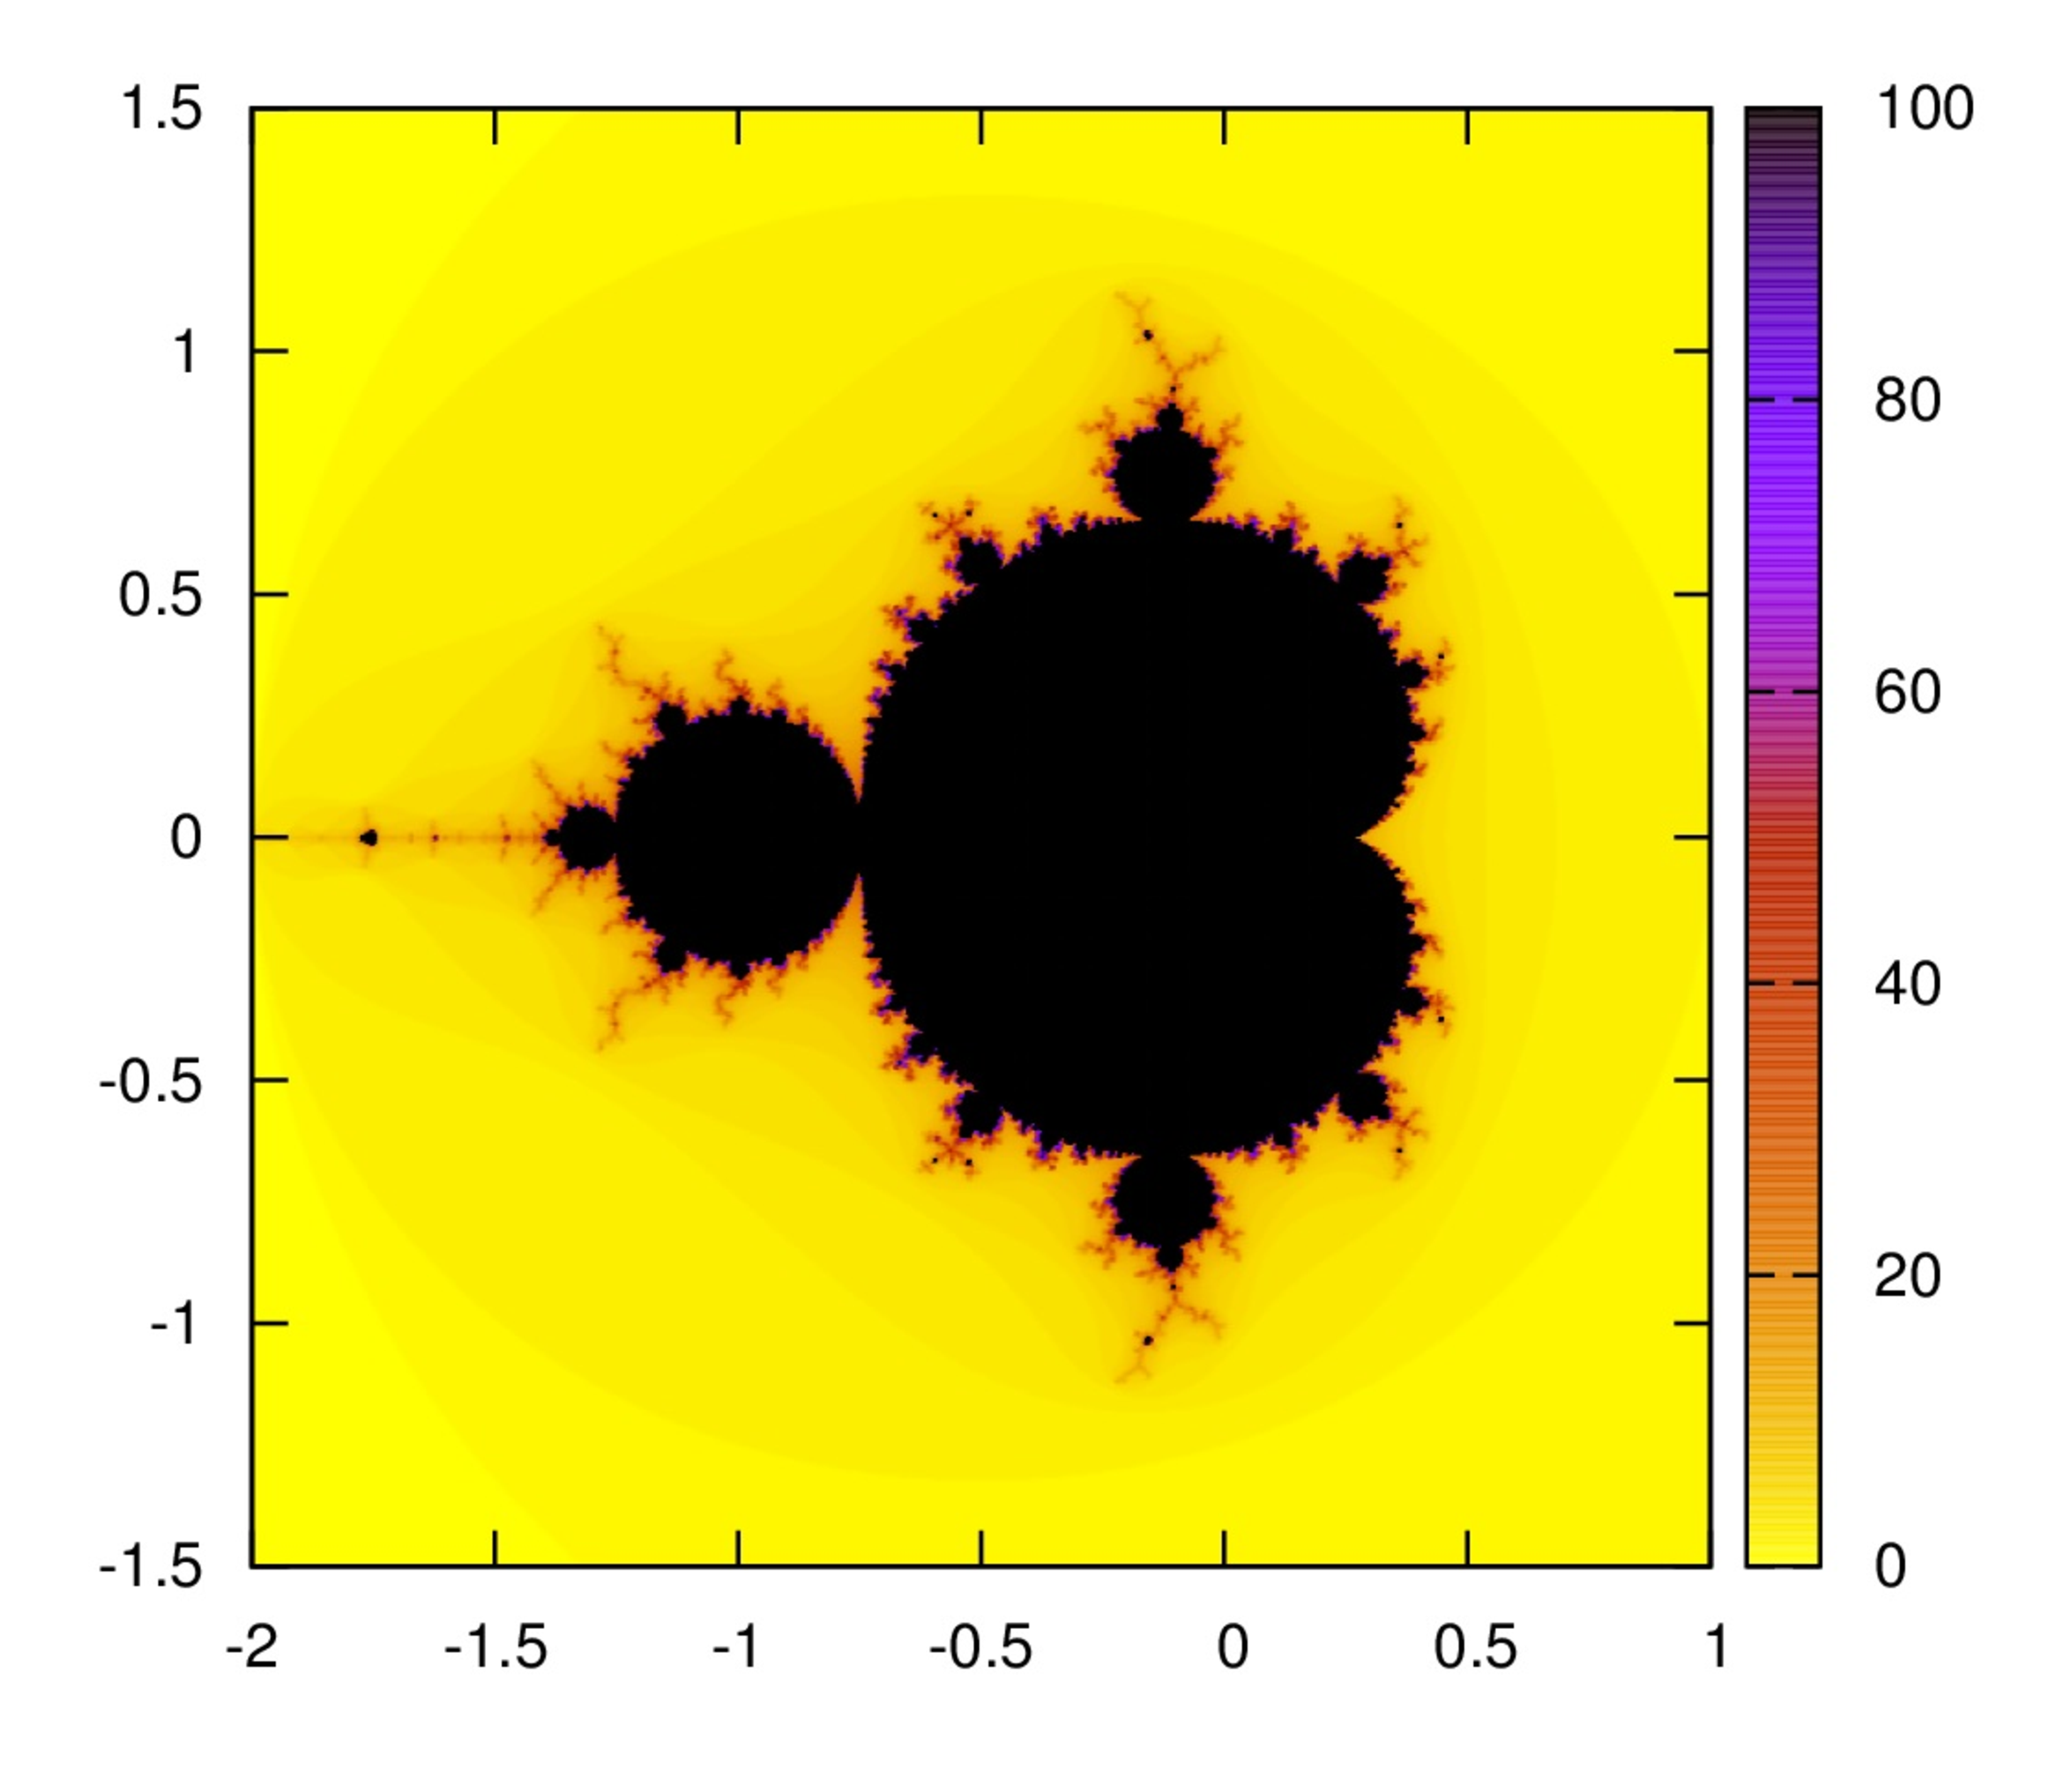
\includegraphics[width=0.75\linewidth]{source/figure/mandel.eps}
\caption{Mandelbrot集合. }
\end{figure}

\subsubsection*{$<$演習課題$>$}
\begin{enumerate}
\item 複素数$c$を与え, $|z_N|>2$を満たす最初の$N$を出力するプログラムを作成せよ. 
\item 上のプログラムを改造して, $-2 \le \Re[c] \le 1, -1.5 \le \Im[c] \le 1.5$の範囲における$N$をファイルに出力せよ. 
また, 出力ファイルをカラーマップで描画せよ. 
\item 図形の一部を解像度を上げて再計算し, Mandelbrot集合がフラクタルであることを確かめよ. 
\end{enumerate}

\subsection{常微分方程式}
一階の微分方程式
\begin{equation}
\frac{dx}{dt}=f(x,t)
\end{equation}
を数値的に解くことを考える. 
計算機は離散的な値しか扱うことができないので, 微分方程式を差分方程式に近似する. 
その最も単純な近似が次のEuler法である. 
\begin{equation}
\frac{x_{n+1}-x_{n}}{\Delta t}=f(x_n,t_n). 
\end{equation}
ここで, $\Delta t$を十分に小さい時間刻み幅として, 
第$n$ステップにおける$t, x$をそれぞれ$t_n(=n \Delta t), x_n$としている. 
初期条件$x(0)=x_0$を与えた上で, $n=0, 1, 2, \cdots$に対して
\begin{equation}
x_{n+1}=x_{n}+f(x_n,t_n)\Delta t
\end{equation}
として逐次$x_n$を求めていく. なお, Taylor展開により,  
\begin{equation}
\begin{split}
x(t+\Delta t)&=x(t)+\frac{dx}{dt}(t)\Delta t+O(\Delta t^2)\\
&=x(t)+f(x,t)\Delta t+O(\Delta t^2)
\end{split}
\end{equation}
であるから, Euler法では1ステップあたり$\Delta t^2$程度の誤差が生じることになる. \\

常微分方程式
\begin{equation}
\frac{dx}{dt}=ax, \ \ \ x(0)=1
\end{equation}
を数値的に解く. なお, この方程式の解は
\begin{equation}
x(t)=\exp(at)
\end{equation}
で与えられる. 

\lstinputlisting[caption={Euler法. }, label=eulermethod]{source/5/EulerMethod.f90}

\subsubsection*{$<$演習課題$>$}
ここに, Euler法の適当な演習課題を一つ追加. 
$\Delta t$を変えたらどうなるか確かめてみる. 

\subsection{Lorenz方程式}
気象学者のLorenzは1963年に熱対流の近似モデルとして
以下の方程式を提案した(Lorenz方程式). 
\begin{equation}
\dfrac{dx}{dt}=-ax+ay, 
\end{equation}
\begin{equation}
\dfrac{dy}{dt}=\mu x-y-xz, 
\end{equation}
\begin{equation}
\dfrac{dz}{dt}=-bz+xy. 
\end{equation}
Lorenzは数値計算により, この方程式の解が
不規則で周期性をもたない振動をすることを発見した. 
このような非周期運動は現在ではカオスと呼ばれている. 

なお, Lorenz方程式は自明解$x=y=z=0$の他に, 
$\mu >1$のとき, 解$x=y=\pm \sqrt{b(\mu-1)}, z=\mu-1$をもつ. 

\begin{figure}[ht]
\centering
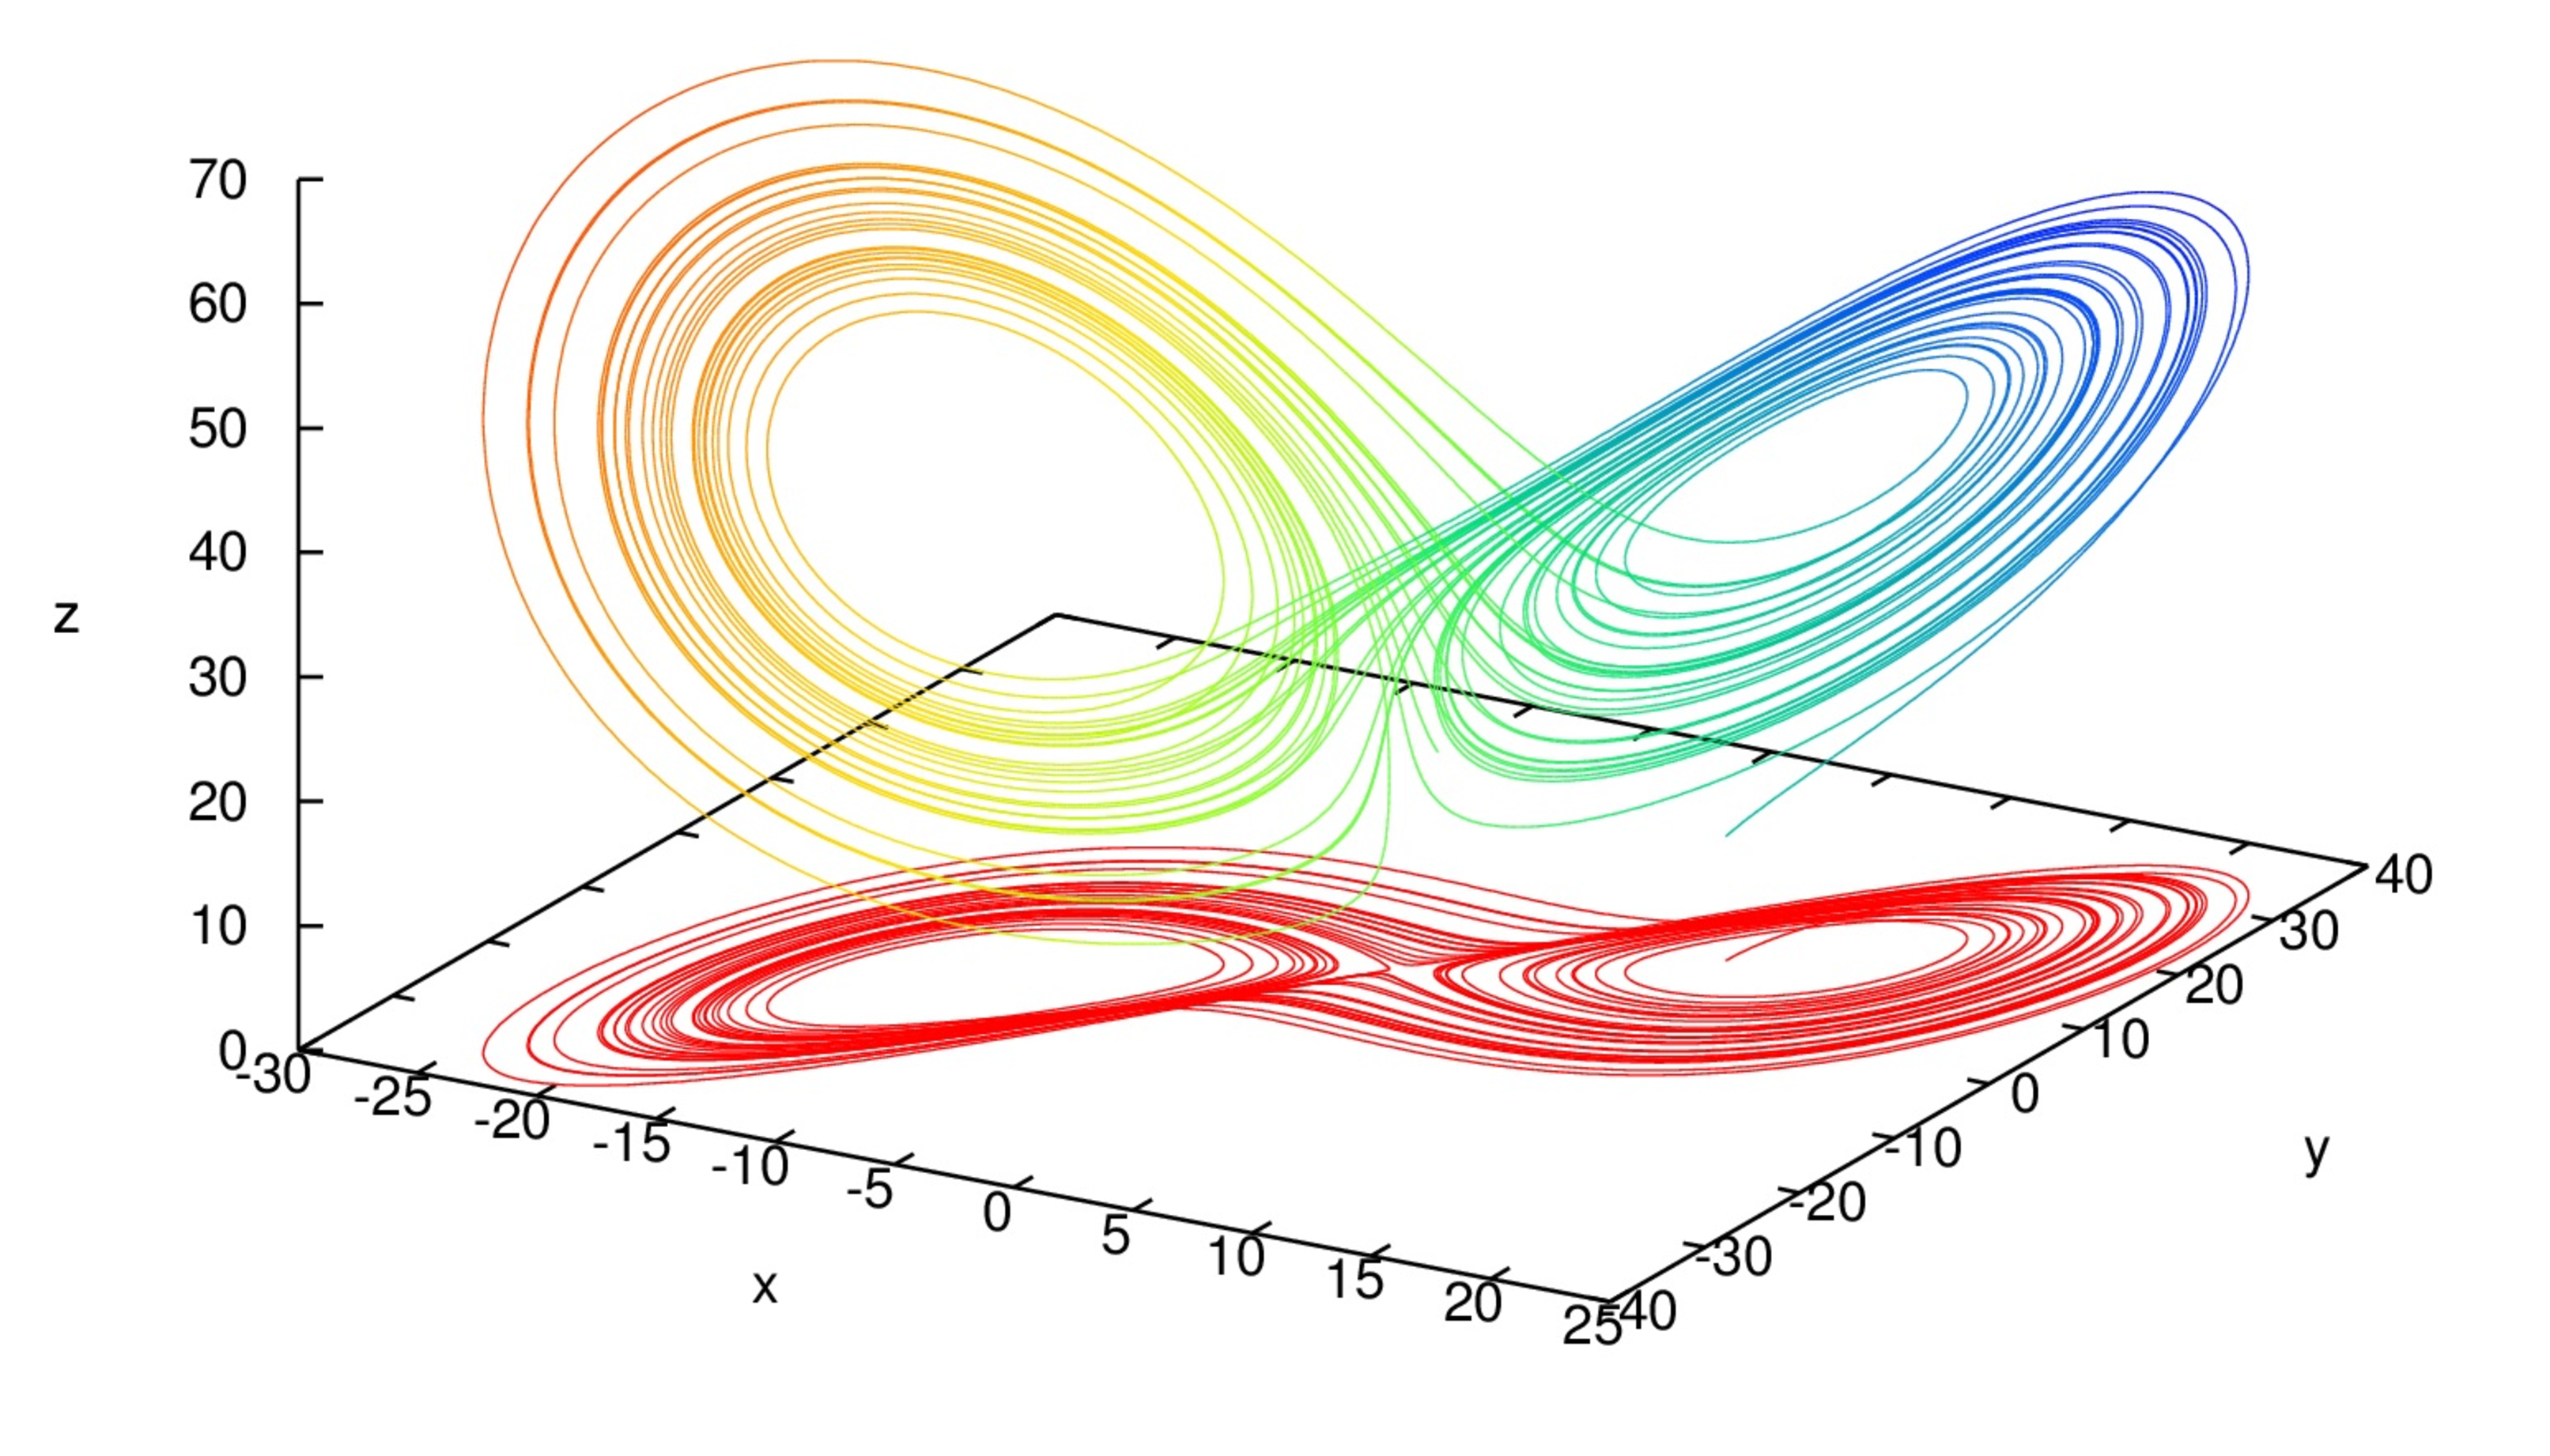
\includegraphics[width=0.9\linewidth]{source/figure/lorenz.eps}
\caption{Lorenzアトラクター. }
\end{figure}

\subsubsection*{$<$演習課題$>$}
\begin{enumerate}
\item $a=10, b=8/3$と固定した上で, Lorenz方程式のシミュレーションを実施せよ. 
$\mu$を徐々に増加させ, どのような解が現れるか調べよ. 
\item 初期値がわずかに(例えば1\%程度)異なる2ケースのシミュレーション結果を比較せよ. 

\end{enumerate}


\subsection{運動方程式}
質点の自由落下をシミュレーションする. 
質点の質量を$m$, 重力加速度を$g$, 初期位置を$h$, 初速を$u_0$とする. 
鉛直座標として$x$をとると, 運動方程式は
\begin{equation}
m\frac{d^2x}{dt^2}=-mg, \ \ \ x(0)=h, \ \ \ \frac{dx}{dt}(0)=u_0
\label{eq_freefall}
\end{equation}
で与えられ, その解は次で与えられる. 
\begin{equation}
x(t)=h+u_0t-\frac{1}{2}gt^2. 
\end{equation}

式(\ref{eq_freefall})を以下のように変形することで一階の連立微分方程式が得られる. 
\begin{equation}
\frac{dx}{dt}=u, \ \ \ x(0)=h, 
\end{equation}
\begin{equation}
\frac{du}{dt}=-g, \ \ \ u(0)=u_0. 
\end{equation}
これをEuler法を用いて数値的に解けばよい. 
プログラムの例を以下に示す. 
\lstinputlisting[caption={質点の自由落下シミュレーション. }, label=freefall]{source/6/FreeFall.f90}



続いて, 質点が空気抵抗を受ける場合のシミュレーションをおこなってみよう. 
質点の投射方向は鉛直方向に限定しない(すなわち, 斜方投射). 
以後, $x, y$をそれぞれ水平, 鉛直方向の座標とする. 


球形物体に働く空気抵抗の大きさ$D$は一般に物体の速さ$(U=\sqrt{(dx/dt)^2+(dy/dt)^2})$の二乗に比例するとしてモデル化される: 
\begin{equation}
D=\frac{1}{2}\rho U^2 \pi a^2 C_D. 
\end{equation}
ここで, $\rho$は空気の密度, $a$は球の半径である. 
また, 抗力係数$C_D$はReynolds数$Re=2aU/\nu$ ($\nu$は空気の動粘性係数)
と呼ばれる無次元数の関数であり, 
$5 \times 10^2 < Re < 1 \times 10^5$のとき約0.44で一定であることが知られている.  

空気抵抗は速度と逆向きに働くので, これを成分$(D_x, D_y)$に分けて運動方程式を書くと, 
\begin{equation}
m\frac{d^2 x}{dt^2}=-D_x, 
\end{equation}
\begin{equation}
m\frac{d^2 y}{dt^2}=-mg-D_y, 
\end{equation}
\begin{equation}
D_x=\frac{dx/dt}{\sqrt{(dx/dt)^2+(dy/dt)^2}}D=\frac{1}{2}\rho \pi a^2 C_D\sqrt{\Big(\frac{dx}{dt}\Big)^2+\Big(\frac{dy}{dt}\Big)^2}\frac{dx}{dt}, 
\end{equation}
\begin{equation}
D_y=\frac{dy/dt}{\sqrt{(dx/dt)^2+(dy/dt)^2}}D=\frac{1}{2}\rho \pi a^2 C_D\sqrt{\Big(\frac{dx}{dt}\Big)^2+\Big(\frac{dy}{dt}\Big)^2}\frac{dy}{dt}. 
\end{equation}
となる. 

\if0 %%%%%%%%%%%%%%%%%%%%%%%%%%%%%%%%%%%%%%%%%%%%%%%%%%%%%%%%%%%%%%%
\subsubsection{Reynolds数が小さい場合}
$Re<0.1$のとき, 抗力係数は理論的に
\begin{equation}
C_D=\frac{24}{Re}
\end{equation}
となることが知られている. 

このとき, 運動方程式は
\begin{equation}
m\frac{d^2 x}{dt^2}=-6\pi \rho \nu a \frac{dx}{dt}, 
\end{equation}
\begin{equation}
m\frac{d^2 y}{dt^2}=-mg-6\pi \rho \nu a \frac{dy}{dt}, 
\end{equation}
となり, 抵抗は速さの一乗に比例する. 
比例係数$6\pi \rho \nu a$は物性値と球の大きさによって決まる. 

\begin{table}[h]
\centering
\begin{tabular}{ccc}
\hline
パラメータ & 値 & 備考 \\
\hline
質量$m$ [kg] & - & 適当に与える \\ \hline
半径$a$ [m] & - & 適当に与える \\ \hline
重力加速度$g$ [m/s$^2$] & 9.80665 & - \\ \hline
空気の密度$\rho$[kg/m$^3$] & 1.261 & 280Kの場合 \\
 & 1.176 & 300Kの場合 \\ \hline
空気の動粘性係数$\nu$[m$^2$/s] & 1.395 $\times 10^{-5}$ & 280Kの場合 \\
 & 1.579 $\times 10^{-5}$ & 300Kの場合 \\ \hline
水の密度$\rho$[kg/m$^3$] & 9.999 $\times 10^2$ & 280Kの場合 \\
 & 9.966 $\times 10^2$ & 300Kの場合 \\ \hline
水の動粘性係数$\nu$[m$^2$/s] & 1.436 $\times 10^{-6}$ & 280Kの場合 \\
 & 8.574 $\times 10^{-7}$ & 300Kの場合 \\ \hline
Reynolds数$Re$[-] & $\frac{2aU}{\nu}$ & 計算する \\ \hline
抗力係数$C_D$[-] & $\frac{24}{Re}$ & $Re<0.1$における理論式 \\
& $(\sqrt{\frac{24}{Re}}+0.5407)^2$ & $Re< 6000$における経験式 \\
& $0.44$ & $5 \times 10^2 < Re < 1 \times 10^5$における近似値 \\
& & (この範囲で抵抗は速度の二乗に比例) \\ \hline
スケールハイト$H_\rho$[m] & 8 $\times 10^3$ & 実際は温度によって変化する \\ \hline
\end{tabular}
\end{table}
\fi %%%%%%%%%%%%%%%%%%%%%%%%%%%%%%%%%%%%%%%%%%%%%%%%%%%%%%%%%%%%%%%%

\subsubsection*{$<$演習課題$>$}
\begin{enumerate}
\item 空気抵抗がない場合($C_D=0$)のシミュレーションをおこない, 解析解と比較せよ. 
\item 空気抵抗がある場合のシミュレーションをおこない, 空気抵抗がない場合と比較せよ. 
もしも$Re$が$5 \times 10^2 < Re < 1 \times 10^5$の範囲になければ警告メッセージを出す仕様にすること. 
\item 空気の温度が変化した場合, 物体の飛距離はどのように変わるか. 
\end{enumerate}

各物理量の具体的な値については, 以下の表を参考にするとよい. 
\begin{table}[h]
\centering
\begin{tabular}{ccc}
\hline
パラメータ & 値 & 備考 \\
\hline
質量$m$ [kg] & - & 適当に与える \\ \hline
半径$a$ [m] & - & 適当に与える \\ \hline
重力加速度$g$ [m/s$^2$] & 9.80665 & - \\ \hline
空気の密度$\rho$[kg/m$^3$] & 1.261 & 280Kの場合 \\
 & 1.176 & 300Kの場合 \\ \hline
空気の動粘性係数$\nu$[m$^2$/s] & 1.395 $\times 10^{-5}$ & 280Kの場合 \\
 & 1.579 $\times 10^{-5}$ & 300Kの場合 \\ \hline
Reynolds数$Re$[-] & - & $2aU/\nu$ \\ \hline
抗力係数$C_D$[-] & $0.44$ & $5 \times 10^2 < Re < 1 \times 10^5$のとき \\ \hline
\end{tabular}
\end{table}



\subsection{素数探索}
素数とは1と自分以外に約数をもたない自然数のことである. 
計算機を用いて数多くの素数を求めてみよう. 

\subsubsection*{$<$演習課題$>$}
\begin{enumerate}
\item 適当な自然数$n$を与え, $2$から$n-1$までの自然数で割り算をおこなうことで
$n$が素数かどうかを判定するプログラムを作成せよ. 
\item 上のプログラムを改造し, 10,000個の素数を探索するプログラムを作成せよ. 
\item アルゴリズムを工夫して, 10,000個の素数を探索するプログラムの高速化をせよ. 
もとのプログラムの何倍速くなったか. 
\end{enumerate}

プログラムの実行時間の測定には, system\_clock関数を用いる. 
その利用法は以下のプログラムを参照せよ. 
\lstinputlisting[caption={実行時間の測定. }, label=timing]{source/7/Timing.f90}


\section{科学技術プレゼンテーション}
\subsubsection*{$<$演習課題$>$}
これまでに取り組んだ数値計算課題(Mandelbrot集合, Lorenz方程式, 斜方投射, 素数探索)
の中から一つテーマを選び, その内容を説明するスライドをPowerPointを用いて作成せよ. 
スライドには以下の内容を含めること. 
\begin{enumerate}
\item タイトルページ
\item 導入, 問題の背景
\item 解く問題の説明, 方程式
\item 計算の手法
\item 計算結果を示す図表
\item 結論, まとめ
\end{enumerate}

\appendix
\section{gfortranのインストール}
gfortranはフリーのコンパイラであるから, 
自分のもっているノートPCや家にあるPCにインストールしておくのがよい. 
その手順を以下に記す. 

\begin{enumerate}
\item https://sourceforge.net/projects/mingw-w64/ にアクセスし, mingw-w64-install.exeをダウンロードする. 
\item ダウンロードしたmingw-w64-install.exeを実行する. 
\item 図\ref{fig_install}(a)で[Next]を押す. 
\item 図\ref{fig_install}(b)でVersionは5.2.0以降, Architectureは64bitマシンの場合はx86\_64を選択する. それ以外の項目はデフォルトでよい. 
\item 図\ref{fig_install}(c)でインストール先を聞かれるが, デフォルトでよい. 
\item 図\ref{fig_install}(d)のようにインストールが始まるのでしばらく待つ.  
\item 図\ref{fig_install}(e)で[Next]を押す. 
\item 図\ref{fig_install}(f)の画面が出たらインストールは終了である. 
\item インストールしたgfortranをコマンドプロンプトから実行するにはgfortranをインストールしたディレクトリにパスを通しておく必要がある.
\textcolor{red}{環境変数の設定を失敗するとシステムが正常に動作しなくなる可能性がある. 自己責任で慎重におこなうこと. }

[コントロールパネル]$\to$[システム]$\to$[システムの詳細設定]$\to$[環境変数]を開く. 
\item システム環境変数中のPathを選択し, [編集]を押す. 
\item 変数値の末尾にセミコロン(;)を挿入し, 続けて各自がgfortranをインストールしたディレクトリを追加する. 
アドレスバーをコピーし, そのまま貼り付けるのがよい. 次はその例である. 

C:Y\llap{=}Program FilesY\llap{=}mingw-w64Y\llap{=}x86\_64-6.1.0-posix-seh-rt\_v5-rev0Y\llap{=}mingw64Y\llap{=}bin

\item コマンドプロンプトを立ち上げ, gfortranとタイプする. 画面に no input files と表示されれば, 正しくパスが通っている. 
\end{enumerate}

\begin{figure}[ht]
\centering
\subfloat[]{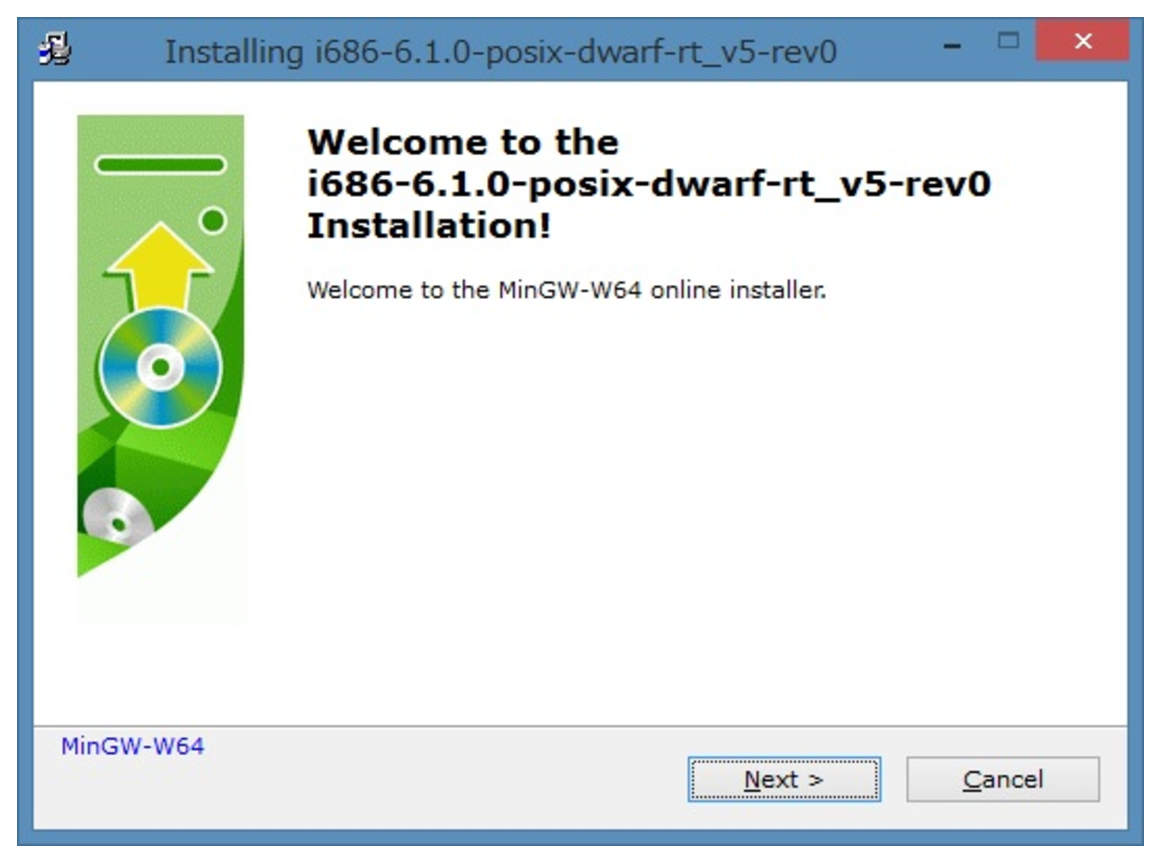
\includegraphics[width=0.45\linewidth]{source/install/1/install1.eps}} \hspace{5mm}
\subfloat[]{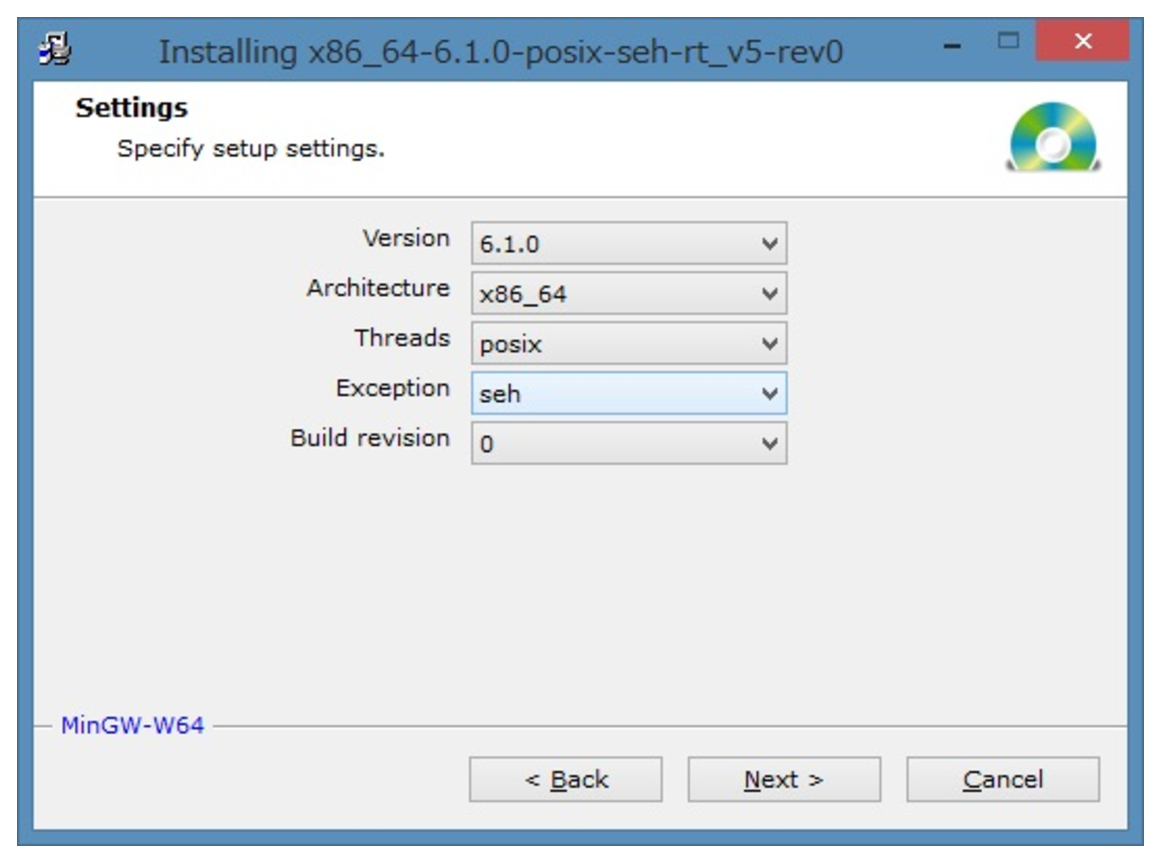
\includegraphics[width=0.45\linewidth]{source/install/1/install2.eps}}\\
\subfloat[]{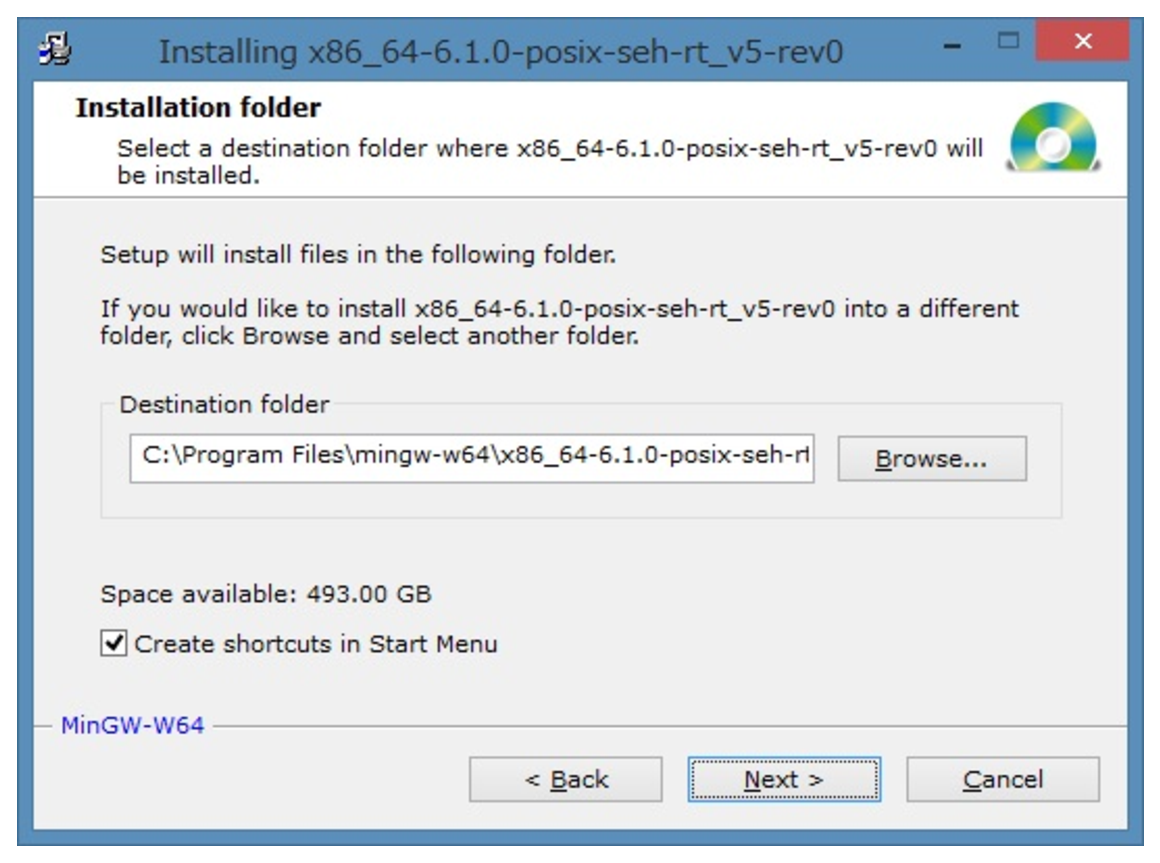
\includegraphics[width=0.45\linewidth]{source/install/1/install3.eps}} \hspace{5mm}
\subfloat[]{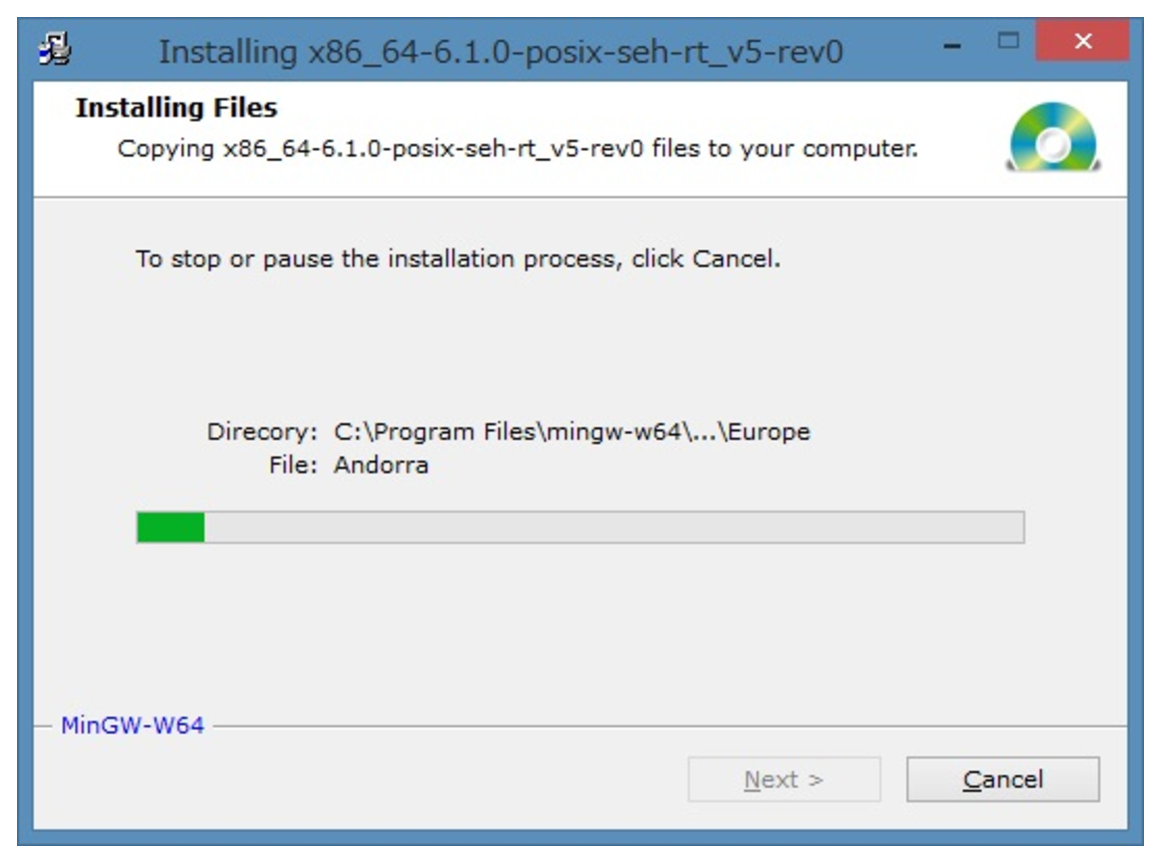
\includegraphics[width=0.45\linewidth]{source/install/1/install4.eps}}\\
\subfloat[]{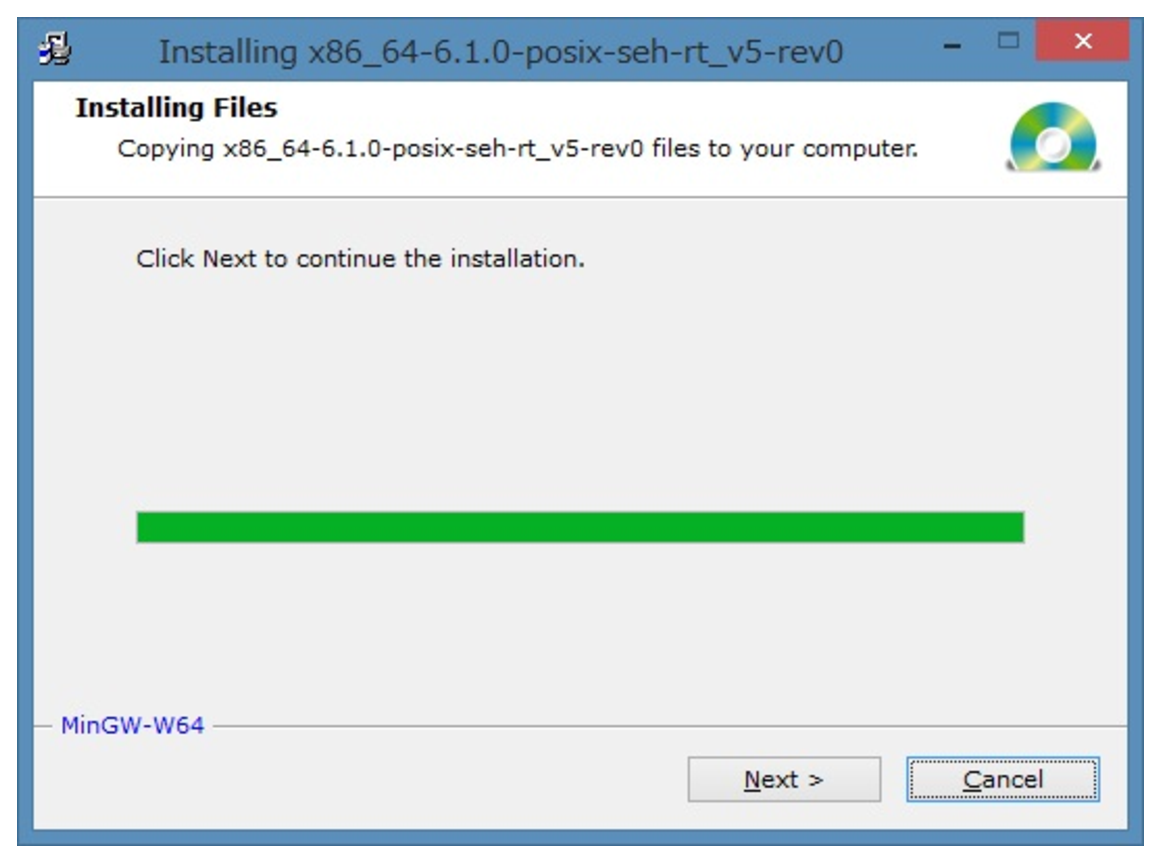
\includegraphics[width=0.45\linewidth]{source/install/1/install5.eps}} \hspace{5mm}
\subfloat[]{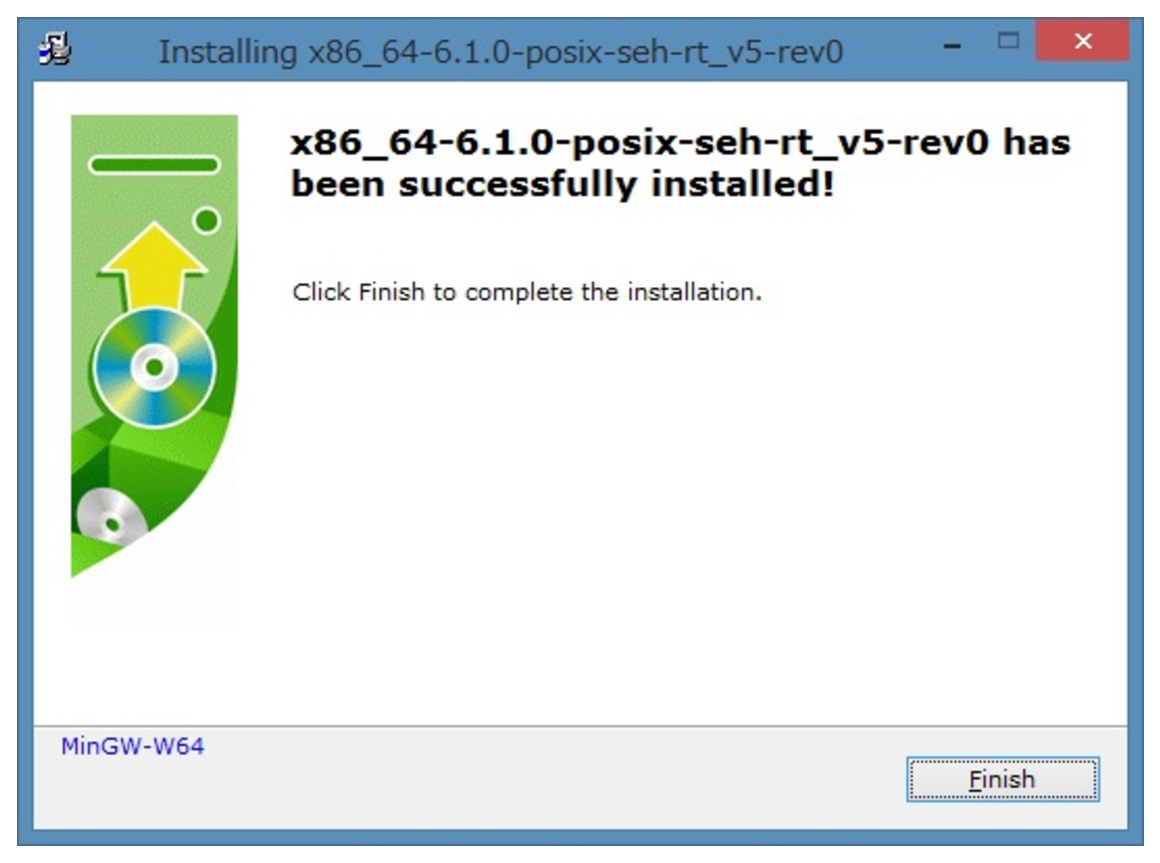
\includegraphics[width=0.45\linewidth]{source/install/1/install6.eps}}\\
\caption{gfotranのインストール.  }
\label{fig_install}
\end{figure}

\clearpage

\section{回答例}

\subsection{Mandelbrot集合}
\lstinputlisting[caption={Mandelbrot集合のプログラム. }, label=mandelbrot_sol]{source/4/Mandelbrot.f90}

\subsection{Lorenz方程式}
\lstinputlisting[caption={Lorenz方程式のEuler法によって解くプログラム. }, label=lorenz_sol]{source/5/Lorenz.f90}

\subsection{斜方投射}
\lstinputlisting[caption={斜方投射のシミュレーションプログラム. }, label=shahou_sol]{source/6/Shahou.f90}

\subsection{素数探索}
\lstinputlisting[caption={素数探索プログラム(簡易版). }, label=prime_sol]{source/7/Prime.f90}
\lstinputlisting[caption={素数探索プログラム(高速版). }, label=primefast_sol]{source/7/PrimeFast.f90}


\end{document}